Der Begriff einer Mannigfaltigkeit basiert per Definition auf lokalen Eigenschaften. Da dennoch sehr h\"aufig globale Eigenschaften von Mannigfaltigkeiten diskutiert werden wollen, wird eine Methode ben\"otigt, aus dem Lokalen ins Globale \"uberzugehen. Eine \"ubliche M\"oglichkeit dies zu tun, ist die Teilung der Eins, mit welchem gewisse lokale Eigenschaften aufrecht erhalten werden, und so immer weiter zu einem globalen Ergebnis erg\"anzt werden k\"onnen. Dies k\"onnte bereits aus der Integrationstheorie auf Untermannigfaltigkeiten des \({\mathbb{R}^n}\) bekannt sein, in dem das gleiche Konzept genutzt wurde, um das Integral auf Mannigfaltigkeiten zu definieren.

\begin{definition}[Teilung der Eins]
    \label{def:part_one:part_one}
    Sei \({\mathfrak{U}=\left(U_i\right)_{i\in I}}\) offene \"Uberdeckung einer Mannigfaltigkeit \({\mathcal{M}}\). Eine Familie von Funktionen \({\theta_i\colon\mathcal{M}\to[0,1],\,i\in I}\) derart, dass
    \begin{enumerate}
        \item \({\theta_i\big|_{\mathcal{M}\setminus U_i}=0}\)
        \item \({\sum_{i\in I}\theta_i=1}\)
    \end{enumerate}
\end{definition}
\"Ahnlich, wie in der Integrationstheorie verlangt wird, dass alle dieser Funktionen integrierbar sind, fordern wir nun, dass alle \({\theta_i}\) differenzierbar sind. Zus\"atzlich werden wir verlangen dass alle Tr\"ager \({\text{supp}(\theta_i)}\) kompakt sind. Wir wollen nun zu einer gegebenen Mannigfaltigkeit eine solche Zerlegung der Eins konstruieren, hierzu ben\"otigen wir den Begriff des guten Atlas.

\section{Gute Atlanten}
\label{sec:part_one:good_atlas}
    \begin{definition}[Untergeordneter guter Atlas]
        \label{def:part_one:good_atlas:good_atlas}
        Sei \({\mathfrak{U}=\left(U_i\right)_{i\in I}}\) offene \"Uberdeckung von \({\mathcal{M}}\). Ein Atlas \({\{\alpha_j\colon B_1\to V_j,\,j\in J\}}\) hei\ss t ein \({\mathfrak{U}}\) untergeordneter guter Atlas, wenn er die folgenden Eigenschaften besitzt:
        \begin{enumerate}
            \item \({\left(V_j\right)_{j\in J}}\) ist eine lokal endliche Verfeinerung von \({\mathfrak{U}}\)\label{def:part_one:good_atlas:good_atlas:0}
            \item \({\left(\alpha_j(B_{\nicefrac{1}{3}})\right)_{j\in J}}\) ist eine offene \"Uberdeckung von \({\mathcal{M}}\)\,.\label{def:part_one:good_atlas:good_atlas:1}
        \end{enumerate}
    \end{definition}
    Hierbei werden zu allen \({V_j}\) differenzierbare Funktionen \({\delta_j\colon V_j\to[0,1]}\) mit 
    \[\delta_i\big|_{\mathcal{M}\setminus V_i}=0\quad\text{und}\quad\delta_i\big|_{\alpha_i\left(B_{\nicefrac{1}{3}}\right)}\not=0\]
    konstruiert. Wegen Eigenschaft 1) ist ihre Summe f\"ur alle \({p\in\mathcal{M}}\) dann endlich, und wegen 2) ungleich null. Die Funktionen
    \[\theta_k:=\frac{\delta_k}{\sum_{i\in I}\delta_i}\]
    bilden eine gew\"unschte Partition der Eins.
    
    \subsection{Erzwingen der \"Uberdeckungseigenschaft endlicher Atlanten}
    \label{sec:part_one:good_atlas:force_cover}
        Obgleich folgendes f\"ur den weiteren Beweis des Einbettungssatzes nicht von weiterer Relevanz sein wird, sei dennoch hier eine M\"oglichkeit aufgezeigt in einem Anwendungsfall (wie unter anderem der Erstellung eines Beispiels zu einer Zerlegung Eins) eine derartige Zerlegung der Eins zu konstruieren. Sei hierzu \({\mathcal{M}}\) eine differenzierbare Mannigfaltigkeit mit einem Atlas \({\{\alpha_i\colon B_1\to\mathcal{M}\}}\). Wir konstruieren Diffeomorphismen \({\mathcal{F}_i\colon B_1\to B_1}\), sodass \({\left\{\left(\alpha_i\circ\mathcal{F}_i\right)\colon B_1\to\mathcal{M}\right\}}\) die Eigenschaft \ref{def:part_one:good_atlas:good_atlas:1} erf\"ullt. Hierf\"ur sei f\"ur \({p\in\mathbb{R}_+}\)
        \[f_p\colon]-\infty,1[\,\to\,]-\infty,1[,\,x\mapsto1-\left(1-x\right)^p\,.\]
        Diese Funktion ist bijektiv, glatt und f\"ur \({x\in[0,1[}\) gilt
        \begin{equation}
            \label{eq:part_one:good_atlas:force_cover:0}
            \lim_{p\to\infty}1-\left(1-x\right)^p=1-0=1\,.
        \end{equation}
        Weiter l\"asst sich ihre Umkehrfunktion leicht bestimmen:
        \[\begin{array}{lrl}
            &f_p(x)=1-\left(1-x\right)^p&=y\\
            \Leftrightarrow&1-y&=\left(1-x\right)^p\\
            \Leftrightarrow&\left(1-y\right)^{\frac{1}{p}}&=1-x\\
            \Leftrightarrow&x&=1-\left(1-y\right)^{\frac{1}{p}}=f_{\nicefrac{1}{p}}(y)\,.
        \end{array}\]
        Demnach ist \({f_p}\) ein \({\mathcal{C}^{\infty}-}\)Diffeomorphismus. Es sei angemerkt, dass dies nur gilt, da die eins nicht im Definitionsbereich enthalten ist. Aufgrund von der Eigenschaft \eqref{eq:part_one:good_atlas:force_cover:0} k\"onnen diese Funktionen nun genutzt werden um eine glatte Funktion \({B_1\to B_1}\) zu definieren, die Kreise mit geringem Radius (z.B. \({r=\nicefrac{1}{3}}\)) auf Kreise mit beliebig gro\ss en Radius \({0<r<1}\) abbildet. Explizit ergibt das die Funktion
        \[F_p\colon B_1\to B_1,\,\mathbf{x}\mapsto\begin{cases}
            0 & \mathbf{x}\not=0\\
            \frac{f_p\left(\norm{\mathbf{x}}\right)}{\norm{\mathbf{x}}}\mathbf{x} & \text{sonst}
        \end{cases}\,.\]
        Es gilt wieder \({F_p^{-1}=F_{\nicefrac{1}{p}}}\), was mithilfe von
        \begin{align*}
            F_{\nicefrac{1}{p}}\left(F_p(\mathbf{x})\right)&=\frac{f_{\nicefrac{1}{p}}\left(\norm{\frac{f_p\left(\norm{\mathbf{x}}\right)}{\norm{\mathbf{x}}}\mathbf{x}}\right)}{\norm{\frac{f_p\left(\norm{\mathbf{x}}\right)}{\norm{\mathbf{x}}}\mathbf{x}}}\frac{f_p\left(\norm{\mathbf{x}}\right)}{\norm{\mathbf{x}}}\mathbf{x}\\
            &=\frac{f_{\nicefrac{1}{p}}\left(\abs{f_p\left(\norm{\mathbf{x}}\right)}\right)}{\abs{f_p\left(\norm{\mathbf{x}}\right)}}\frac{f_p\left(\norm{\mathbf{x}}\right)}{\norm{\mathbf{x}}}\mathbf{x}=\frac{\norm{\mathbf{x}}}{\norm{\mathbf{x}}}\mathbf{x}=\mathbf{x}
        \end{align*}
        aus Symmetriegr\"unden folgt. Hierbei gilt \({\abs{f_p\left(\norm{\mathbf{x}}\right)}=f_p\left(\norm{\mathbf{x}}\right)}\), da \({f_p}\) das Einheitsintervall bijektiv auf sich selbst abbildet. Dies ist gerade die Funktion, die einen Punkt mit Radius \({r}\) auf ein skalares Vielfaches von sich selbst mit Radius \({f_p(r)}\) abbildet. Da \({f_p}\) diffeomorph ist, ist es damit auch \({F_p}\). Unter \({F_p}\) gilt zum Beispiel f\"ur \({r\in\,]0,1[}\)
        \[F_p\left(B_r\right)=B_{f_p\left(r\right)}\mathrel{\big\uparrow_{p=1}^{\infty}}B_1\,.\]
            
        \subsubsection{Konstruktion eines neuen Atlas}
        \label{sec:part_one:good_atlas:force_cover:new_atlas}
            Sei bereits ein beliebiger \textit{endlicher} \({\mathcal{C}^k-}\)Atlas \({\{\beta_i\colon B_1\to U_i\}}\) bekannt. Wegen der Endlichkeit sind beliebige Schnitte der \({U_i}\) erneut offen (eine Schlussfolgerung der \textit{m\"oglicherweise} auch lokale Endlichkeit gen\"ugen w\"urde) sodass stets \({p_i}\) derart existieren, dass die \({\beta_i\circ F_{p_i}}\) die Bedingung \ref{def:part_one:good_atlas:good_atlas:1} erf\"ullen. Definieren wir \({\mathcal{F}_i:=F_{p_i}}\), erhalten wir die gewünschten Karten. Da nun jede Kette von Abbildungen nur so differenzierbar ist wie ihr schw\"achstes Glied, bilden die \({\alpha_i:=\beta_i\circ\mathcal{F}_i}\) erneut einen \({\mathcal{C}^k-}\)Atlas. Die Auswirkung der \({F_p}\) auf die Karten kann in \ref{fig:part_one:good_atlas:force_cover_new_atlas:ex0} erkannt werden.
        
            \begin{figure}
                \centering
                \begin{tikzpicture}
                    \node {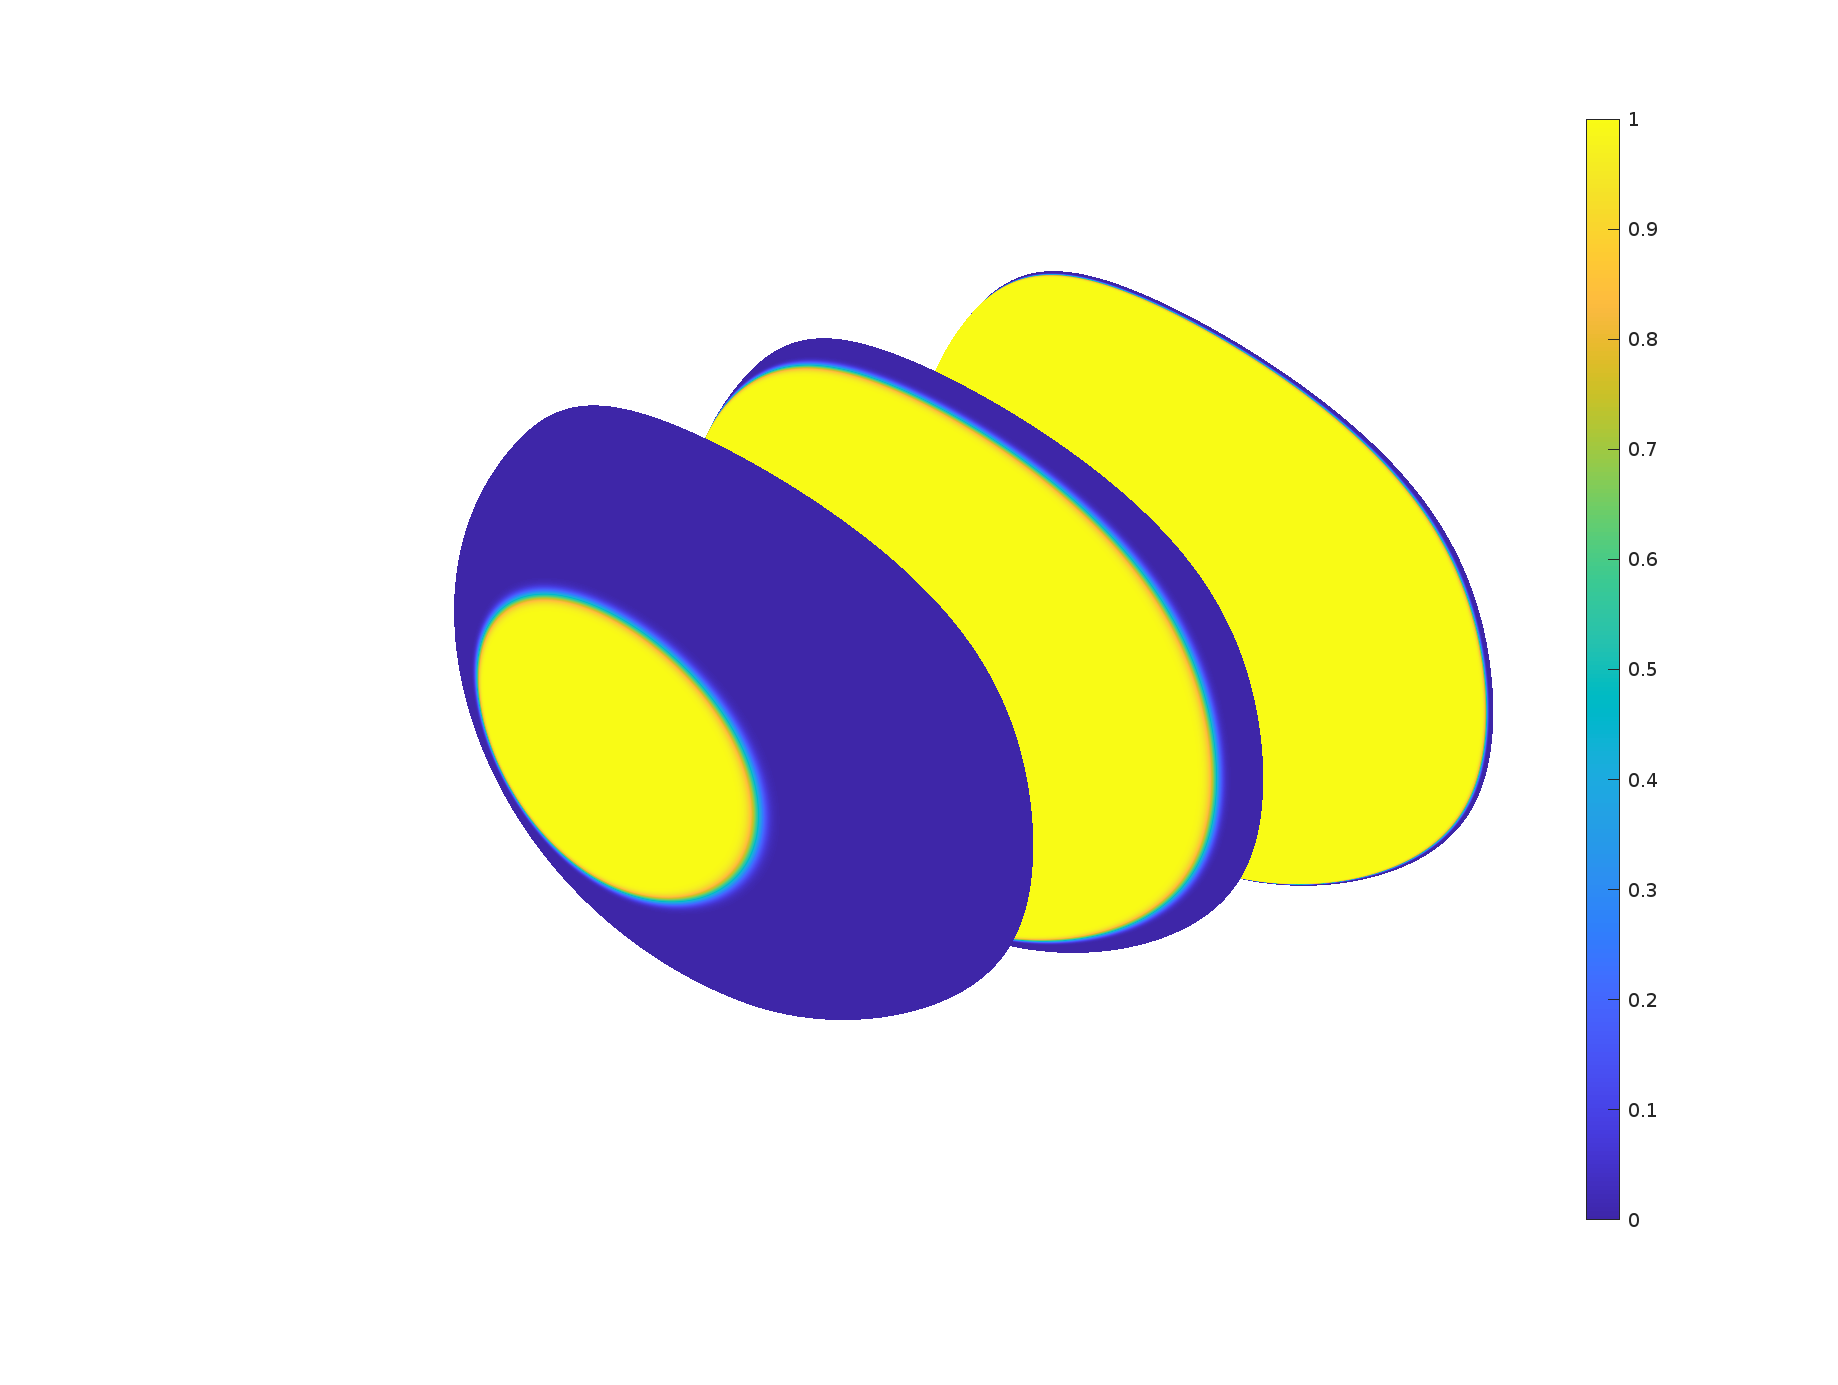
\includegraphics[scale = 0.3]{Images/Exponents.eps}};
                    \node at (0, -2) {\({p=1}\)};
                    \node at (1.2, -1.6) {\({p=4}\)};
                    \node at (2.4, -1.2) {\({p=7}\)};
                \end{tikzpicture}
                \caption{Auswirkung des \({p}\) der \({F_p}\) auf die resultierenden Karten der Konstruktion \ref{sec:part_one:good_atlas:force_cover:new_atlas}.}
                \label{fig:part_one:good_atlas:force_cover_new_atlas:ex0}
            \end{figure}
        
    \subsection{Existenz eines guten Atlas}
    \label{sec:part_one:good_atlas:exists}
        Wir wenden uns nun der Existenz eines guten Atlas zu. Der Beweis beruht grundlegend auf der echt aufsteigenden kompakten \"Uberdeckung aus Lemma \ref{lem:top_man:rel_comp_cover}. Folgende Beweisidee ist in Abbildung \ref{fig:part_one:good_atlas:exist:ex0} dargestellt. 
        Wir wenden uns nun der Existenz eines guten Atlas zu. Der Beweis beruht grundlegend auf der echt aufsteigenden kompakten \"Uberdeckung aus Lemma \ref{lem:top_man:rel_comp_cover}, und verl\"auft \"ahnlich zu dem der Parakompaktheit. Folgende Beweisidee ist in Abbildung \ref{fig:part_one:good_atlas:exist:ex0} dargestellt. 
        \begin{theorem}[Existenz eines guten Atlas]
            \label{thm:part_one:good_atlas:exists:exists}
            Eine differenzierbare Mannigfaltigkeit \({\mathcal{M}}\) besitzt zu jeder beliebigen offenen \"Uberdeckung \({\mathfrak{U}}\) einen untergeordneten guten Atlas.
        \end{theorem}
        \begin{proof}
            Da \({\mathcal{M}}\) lokalkompakt und zweitabz\"ahlbar ist, existiert nach Lemma \ref{lem:top_man:comp_asc_cover} eine echt aufsteigende kompakte \"Uberdeckung \({A_k}\). Seien
            \[S_k^1:=A_k\setminus\mathring{A}_{k-1}\quad\text{und}\quad S_k^2:=A_{k+1}\setminus\mathring{A}_{k-2}\]
            erneut kompakt. Weiter gibt es f\"ur jedes \({\mathbf{y}\in S_k^1}\) eine Karte \({\alpha_{i_{\mathbf{y}}}\colon V_{i_{\mathbf{y}}}\to U_{i_{\mathbf{y}}}}\) mit \({U_{i_{\mathbf{y}}}\subseteq S_k^2}\), sei also \({\mathbf{x}=\alpha^{-1}_{i_{\mathbf{y}}}(\mathbf{y})}\). Da \({\alpha_{i_{\mathbf{y}}}}\) stetig ist, ist das Urbild von \({U_{i_{\mathbf{y}}}\cap\mathring{S}_k^2}\) unter \({\alpha_{i_{\mathbf{y}}}}\) offen (und nicht leer), und wir k\"onnen einen Radius \({\epsilon_{\mathbf{y}}}\) finden, sodass
            \begin{equation}
                \label{eq:part_one:good_atlas:abstr_con:0}
                \Delta_{\mathbf{y}}:=B_{\frac{\epsilon_{\mathbf{y}}}{3}}\left(\mathbf{x}\right)\subset B_{\epsilon_{\mathbf{y}}}\left(\mathbf{x}\right)\subseteq\alpha_{i_{\mathbf{y}}}^{-1}\left(U_{i_{\mathbf{y}}}\cap\mathring{S}_k^2\right)\,.
            \end{equation}
            Die \({\left(\alpha_{i_{\mathbf{y}}}\left(\Delta_{\mathbf{y}}\right)\right)_{\mathbf{y}\in S_k^1}}\) bilden nun offenbar eine offene \"Uberdeckung von \({S_k^1}\). Da \({S_k^1}\) kompakt ist, besitzt diese eine endliche Teil\"uberdeckung, es existiert also eine endliche Teilmenge \({S^{\prime}_k\subset S_k^1}\), sodass
            \begin{equation}
            \label{aaarar}
                S_k^1\subset\bigcup_{\mathbf{z}\in S_k^{\prime}}\alpha_{i_{\mathbf{z}}}\left(\Delta_{\mathbf{z}}\right)\mathop{\subset}^{\eqref{eq:part_one:good_atlas:abstr_con:0}}\mathring{S}_k^2\cap\bigcup_{\mathbf{z}\in S_k^{\prime}}U_{i_{\mathbf{z}}}\subseteq\mathring{S}_k^2
            \end{equation}
            gilt. Wir definieren
            \[\beta_{\mathbf{y}}\colon B_1\to\alpha_{i_{\mathbf{y}}}\left(B_{\epsilon_{\mathbf{y}}}\right),\,\mathbf{z}\mapsto\alpha_{i_{\mathbf{y}}}\left(\epsilon_{\mathbf{y}}\cdot\mathbf{z}\right)\hspace{1.5cm}\forall\mathbf{y}\in S_k^{\prime}\,,\]
            und erhalten letztenendes mit
            \[\left\{\beta_{\mathbf{y}}\colon B_1\to\alpha_{i_{\mathbf{y}}}\left(B_{\epsilon_{\mathbf{y}}}\right)\big|\,\forall\mathbf{y}\in S_k^{\prime}\colon\forall k\in\mathbb{N}\right\}\]
            den gesuchten abz\"ahlbaren Atlas. Die lokale Endlichkeit folgt dabei aus \ref{aaarar}.
        \end{proof}
    
        \begin{figure}
            \centering
            \fbox{
            \small
            \begin{tikzpicture}[scale = 1.4]
    
                \draw   (165:4) node at +(-1, 1) (c1) {}
                        (165:4) node at +(1, -1) (c2) {}
                        (130:4) node at +(1, 0) (c3) {};
                        
                \begin{scope}[line width = 0pt]
                
                    \path [pattern = north east lines] 
                        (0, 4) arc (90:180:4) -- (-3, 0) arc (180:90:3) -- cycle
                        (0, 2) arc (90:180:2) -- (-1, 0) arc (180:90:1) -- cycle;
                        
                    \path [pattern = north west lines] 
                        (0, 3) arc (90:180:3) -- (-2, 0) arc (180:90:2) -- cycle;
                    
                    \fill [white]
                        (130:4) .. controls ++(-1, 0) and (c1) .. (165:4)
                        .. controls (c2) and (-0.5, 1) .. (-1.5, 1.5)
                        .. controls (-2.5, 2) and (c3) .. (130:4) -- cycle;
           
                \end{scope}
    
                \draw
                    \foreach\r in {1,2,3,4}{ (0, \r) arc (90:180:\r) }
                    
                    (-3, 0.8) .. controls (-2.2, 0.4) and (-2, 0.8) .. (-2.4, 1.2)
                    .. controls (-2.8, 1.6) and (-2, 2.8) .. (-2.8, 2.4)
                    .. controls (-3.6, 2) and (-3.8, 1.2) .. (-3, 0.8)% node [pos = 0, above, sloped] {\({U_{i_{\mathbf{x}}}}\)}
                    
                    (-2.7, 0.8) .. controls (-2.5, 0.7) and (-2.4, 0.8) .. (-2.5, 1.1)
                    .. controls (-2.6, 1.4) and (-2.5, 2.3) .. (-3, 1.8)% node [pos = 0.9, above, sloped] {\({U_{i_{\mathbf{x}}}}\)}
                    .. controls (-3.5, 1.3) and (-2.9, 0.9) .. (-2.7, 0.8)
                    
                    (1, 1.5) .. controls (1.4, 1.6) and (1.6, 2.8) .. (2.2, 2.6)
                    
                    (-2.7, 1) node {\tiny\textbullet}
                    (2, 1) node {\tiny\textbullet}
                    ++(2/9, 0) arc (0:360:2/9) node [pos = 0.125, sloped, above] {\({\Delta_{\mathbf{x}}}\)}
                    ++(4/9, 0) arc (0:360:2/3) node [pos = 0.125, sloped, above] {\({B_{\epsilon_{\mathbf{x}}}}\)}
                    
                    (2, 4) node {\({\mathbb{R}^n}\)}
                    (-2.7, 4) node {\({\mathcal{M}}\)};
                
                \begin{scope}[line width = 1pt]
                    \draw [dashed, line width = 1pt] 
                        (130:4) .. controls ++(-1, 0) and (c1) .. (165:4) node [pos = 0.3, above, sloped] {\({U_{i_{\mathbf{x}}}}\)}
                        (2.2, 2.6) .. controls (1.2, 3.4) and (1, 2.5) .. (1, 1.5);
        
                    \draw (1, 1.5) .. controls (1, 0.5) and (1.5, 0) .. (2.6, 0.4)
                        .. controls (3.7, 0.8) and (3.2, 1.8) .. (2.2, 2.6) node [pos = 0.75, sloped, above] {\({V_{i_{\mathbf{x}}}}\)}
                        (165:4) .. controls (c2) and (-0.5, 1) .. (-1.5, 1.5)
                        .. controls (-2.5, 2) and (c3) .. (130:4);
                \end{scope}
    
                        
                \draw [decorate, decoration = {calligraphic brace, raise=3pt, amplitude = 5pt}] (-2, 0) -- node [below = 5pt] {\({S_k^1}\)} (-3, 0);
                \draw [decorate, decoration = {calligraphic brace, raise=18pt, amplitude = 10pt}] (-1, 0) -- node [below = 25pt] {\({S_k^2}\)} (-4, 0);
    
                \draw [->] (1.75, 1.25) [bend right] to node [pos = 0.3, above] {\({\alpha_{i_{\mathbf{x}}}}\)} (-2.4, 1.25);
            \end{tikzpicture}
            }
            \caption{Konstruktion eines guten Atlas}
            \label{fig:part_one:good_atlas:exist:ex0}
        \end{figure}

\section{Konstruktion einer Zerlegung der Eins}
\label{sec:part_one:constr_one}
    Ein gegebener guter Atlas erm\"oglicht uns nun, eine Zerlegung der Eins zu konstruieren. Sei hierzu zun\"achst
    \[\lambda\colon\mathbb{R}\to[0,1[,\,t\mapsto\begin{cases}
        e^{-\frac{1}{t^2}} & t>0\\
        0 & \text{sonst}
    \end{cases}\,.\]
    Man sieht, dass die Ableitung dieser Funktion 
    \[\frac{\text{d}^n\lambda}{\text{d}^nt}=r_n(t)\lambda(t)\]
    mit einer rationalen Funktion \({r_n}\) ist. Wir zeigen mittels Induktion, dass \({\lambda}\) glatt ist. Sowohl der Induktionsanfang als auch der Induktionsschritt folgen aus
    \[\lambda^{(n)}(0)=\lim_{\genfrac{}{}{0pt}{}{h\to0}{h\not=0}}\frac{\lambda^{(n-1)}(h)-\lambda^{(n-1)}(0)}{h}=\lim_{\genfrac{}{}{0pt}{}{h\to0}{h\not=0}}\frac{r_{n-1}(h)e^{-\frac{1}{h^2}}-0}{h}=0\,.\]
    Der Tr\"ager von \({\lambda}\) ist \({\text{supp}(\lambda)=\mathbb{R}_{\geq0}}\). Wir setzen nun
    \[\phi\colon\mathbb{R}\to[0,1],\,t\mapsto\frac{\lambda(t)}{\lambda(t)+\lambda(1-t)}\,,\]
    sodass wir eine differenzierbare Funktion erhalten, die f\"ur \({t\leq0}\) verschwindet und f\"ur \({t\geq1}\) gleich eins ist. Sei weiter
    \[\psi\colon\mathbb{R}^n\to[0,1],\,\mathbf{x}\mapsto1-\phi\left(3\norm{\mathbf{x}}-1\right)\,,\]
    eine Funktion mit Tr\"ager \({\overline{B_{\nicefrac{2}{3}}}}\). Wir definieren f\"ur \({i\in\Lambda}\) die Funktionen
    \[\omega_i\colon\mathcal{M}\to[0,1],\,\mathbf{x}\mapsto\begin{cases}
        \left(\psi\circ\alpha_i^{-1}\right)(\mathbf{x}) & \mathbf{x}\in\alpha_i\left(B_{\nicefrac{2}{3}}(0)\right)\\
        0 & \text{sonst}
    \end{cases}\,,\]
    die aufgrund der lokalen Endlichkeit summierbar sind - f\"ur jedes \({\mathbf{x}\in\mathcal{M}}\) sind lediglich endlich viele \({\omega_i(\mathbf{x})\not=0}\). Da die \({\alpha_i\left(B_{\nicefrac{2}{3}}(0)\right)}\) immer noch eine \"Uberdeckung von \({\mathcal{M}}\) bilden, ist die Summe au\ss erdem \"uberall ungleich null. Wir erhalten final die nun wohldefinierten
    \[\theta_i:=\frac{\omega_i}{\sum_{j\in\Lambda}\omega_j}\,,\]
    die wegen
    \[\sum_{i\in\Lambda}\theta_i=\frac{\sum_{i\in\Lambda}\omega_i}{\sum_{j\in\Lambda}\omega_j}=1\]
    eine Teilung der Eins darstellen. Da der Nenner stets mindestens so gro\ss{} wie der Z\"ahler ist, ist zudem \({0<\theta_i\leq 1}\).
    
\section{Beispiel Teilung der Eins}
\label{sec:part_one:ex0}
    Bezeiche im Folgenden stets
    \[E_{a,b}=\left\{\mathbf{x}\in\mathbb{R}^2\colon\sqrt{\left(\frac{x_1}{a}\right)^2+\left(\frac{x_2}{b}\right)^2}\leq1\right\}\]
    die Ellipse mit Radien \({a}\) und \({b}\).
    Wir betrachten die Nullstellenmenge des Gleichungssystems
    \begin{align}
        \cos(x)+\cos(y)-z^2&=1
    \end{align}
    im \({\mathbb{R}^3}\). Sei \({\mathcal{M}}\) die Zusammenhangskomponente nahe des Ursprungs. L\"osen wir jeweils in eine Richtung auf, erhalten wir naiv sechs Karten. Mit den Bezeichnungen \({U=\{0<\cos(x)-y^2\leq1\}}\) und \({V=\{1<\cos(x)+\cos(y)\leq2\}}\) ergeben sich explizit
    \[\gamma_{1,2}\colon U\to\mathcal{M},\mathbf{x}\mapsto\left(\pm\arccos\left(\cos(x)-y^2-1\right),x,y\right)^T\]
    \[\gamma_{3,4}\colon U\to\mathcal{M},\mathbf{x}\mapsto\left(x,\pm\arccos(\cos(x)-y^2-1),y\right)^T\]
    \[\gamma_{5,6}\colon V\to\mathcal{M},\mathbf{x}\mapsto\left(x,y,\pm\sqrt{\cos(x)+\cos(y)-1}\right)^T\,.\]
    Obgleich es sicher scheint, dass \({B_1}\), \({U}\) und \({V}\) zueinander diffeomorph sind, ist es nicht einfach explizite Diffeomorphismen anzugeben. Anstelle dessen betrachten wir die hinreichend gro\ss en einfacheren Teilmengen \({E_{\nicefrac{3}{2},\nicefrac{9}{10}}\subset U}\) und \({B_{\nicefrac{4}{3}}\subset V}\) und die induzierten Karten
    \[\beta_i:=\begin{cases}
        \gamma_i\mathrel{|}_{E_{\nicefrac{3}{2},\nicefrac{9}{10}}} & 1\leq i\leq4\\
        \gamma_i\mathrel{|}_{B_{\nicefrac{4}{3}}} & \text{sonst}
    \end{cases}\,,\]
   die immer noch einen Atlas von \({\mathcal{M}}\) bilden (ohne Beweis). Da der Atlas endlich ist, k\"onnen wir Wie in Sektion \ref{sec:part_one:good_atlas:force_cover} beschrieben erhalten wir aus den \({\beta_i}\) nun einen Atlas \({\{\alpha_i\to M\}}\), der aufgrund der Endlichkeit des vorherigen Atlas auch gut ist. Dieser, und die von ihm implizierte Teilfunktionen der Zerlegung der eins sind in Abbildung \ref{fig:part_one:good_atlas:exist:ex0} dargestellt.
    
    \begin{figure}
        \centering
        \begin{subfigure}{0.49\textwidth}
            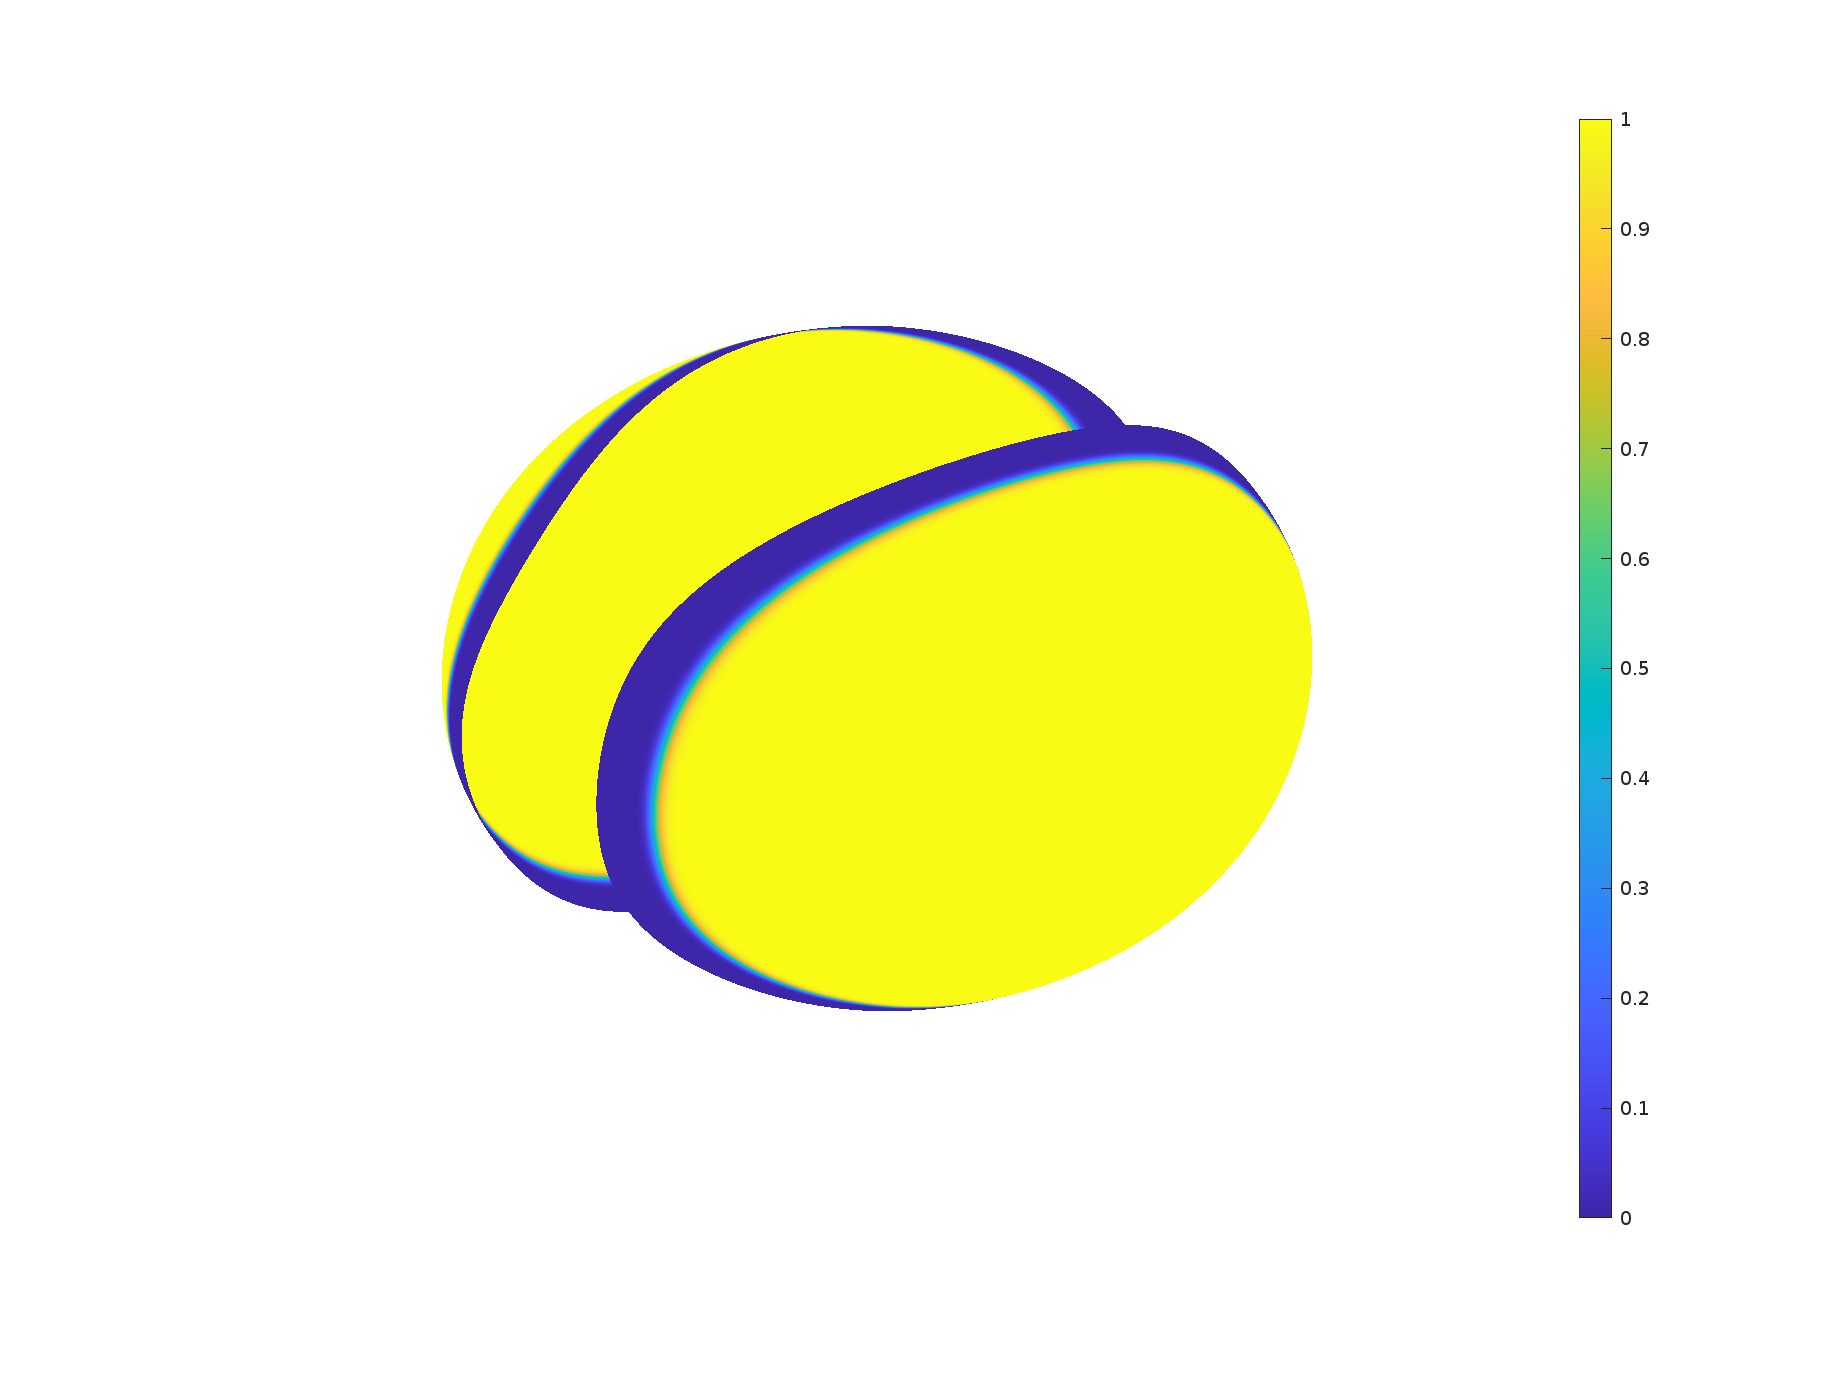
\includegraphics[scale = 0.2]{Images/PoO_01.eps}
            \caption{Die Karten \({\alpha_1}\) und \({\alpha_2}\).}
        \end{subfigure}
        \begin{subfigure}{0.49\textwidth}
            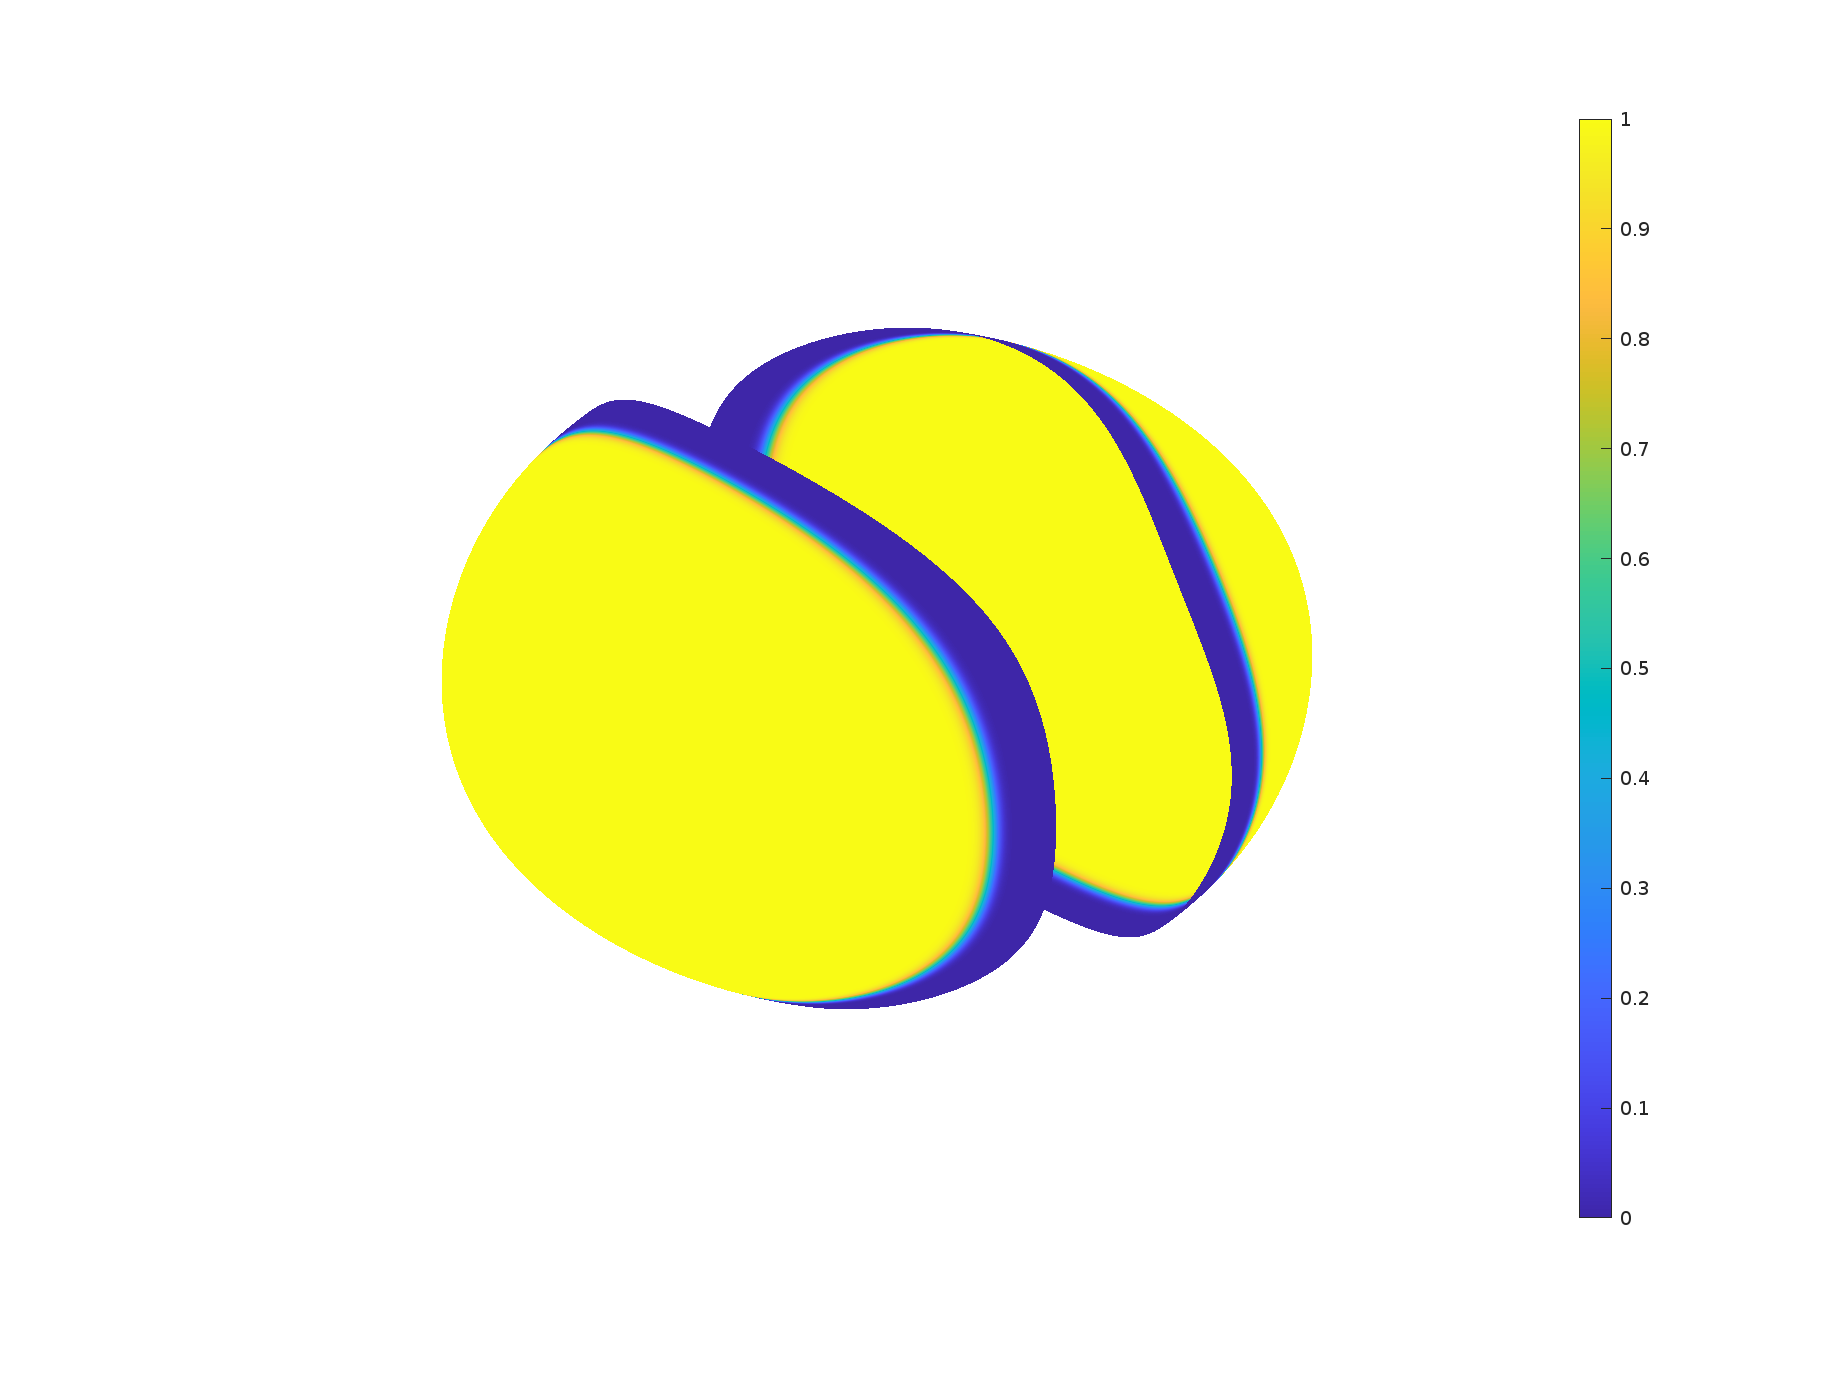
\includegraphics[scale = 0.2]{Images/PoO_02.eps}
            \caption{Die Karten \({\alpha_3}\) und \({\alpha_4}\).}
        \end{subfigure}
        \begin{subfigure}{0.49\textwidth}
            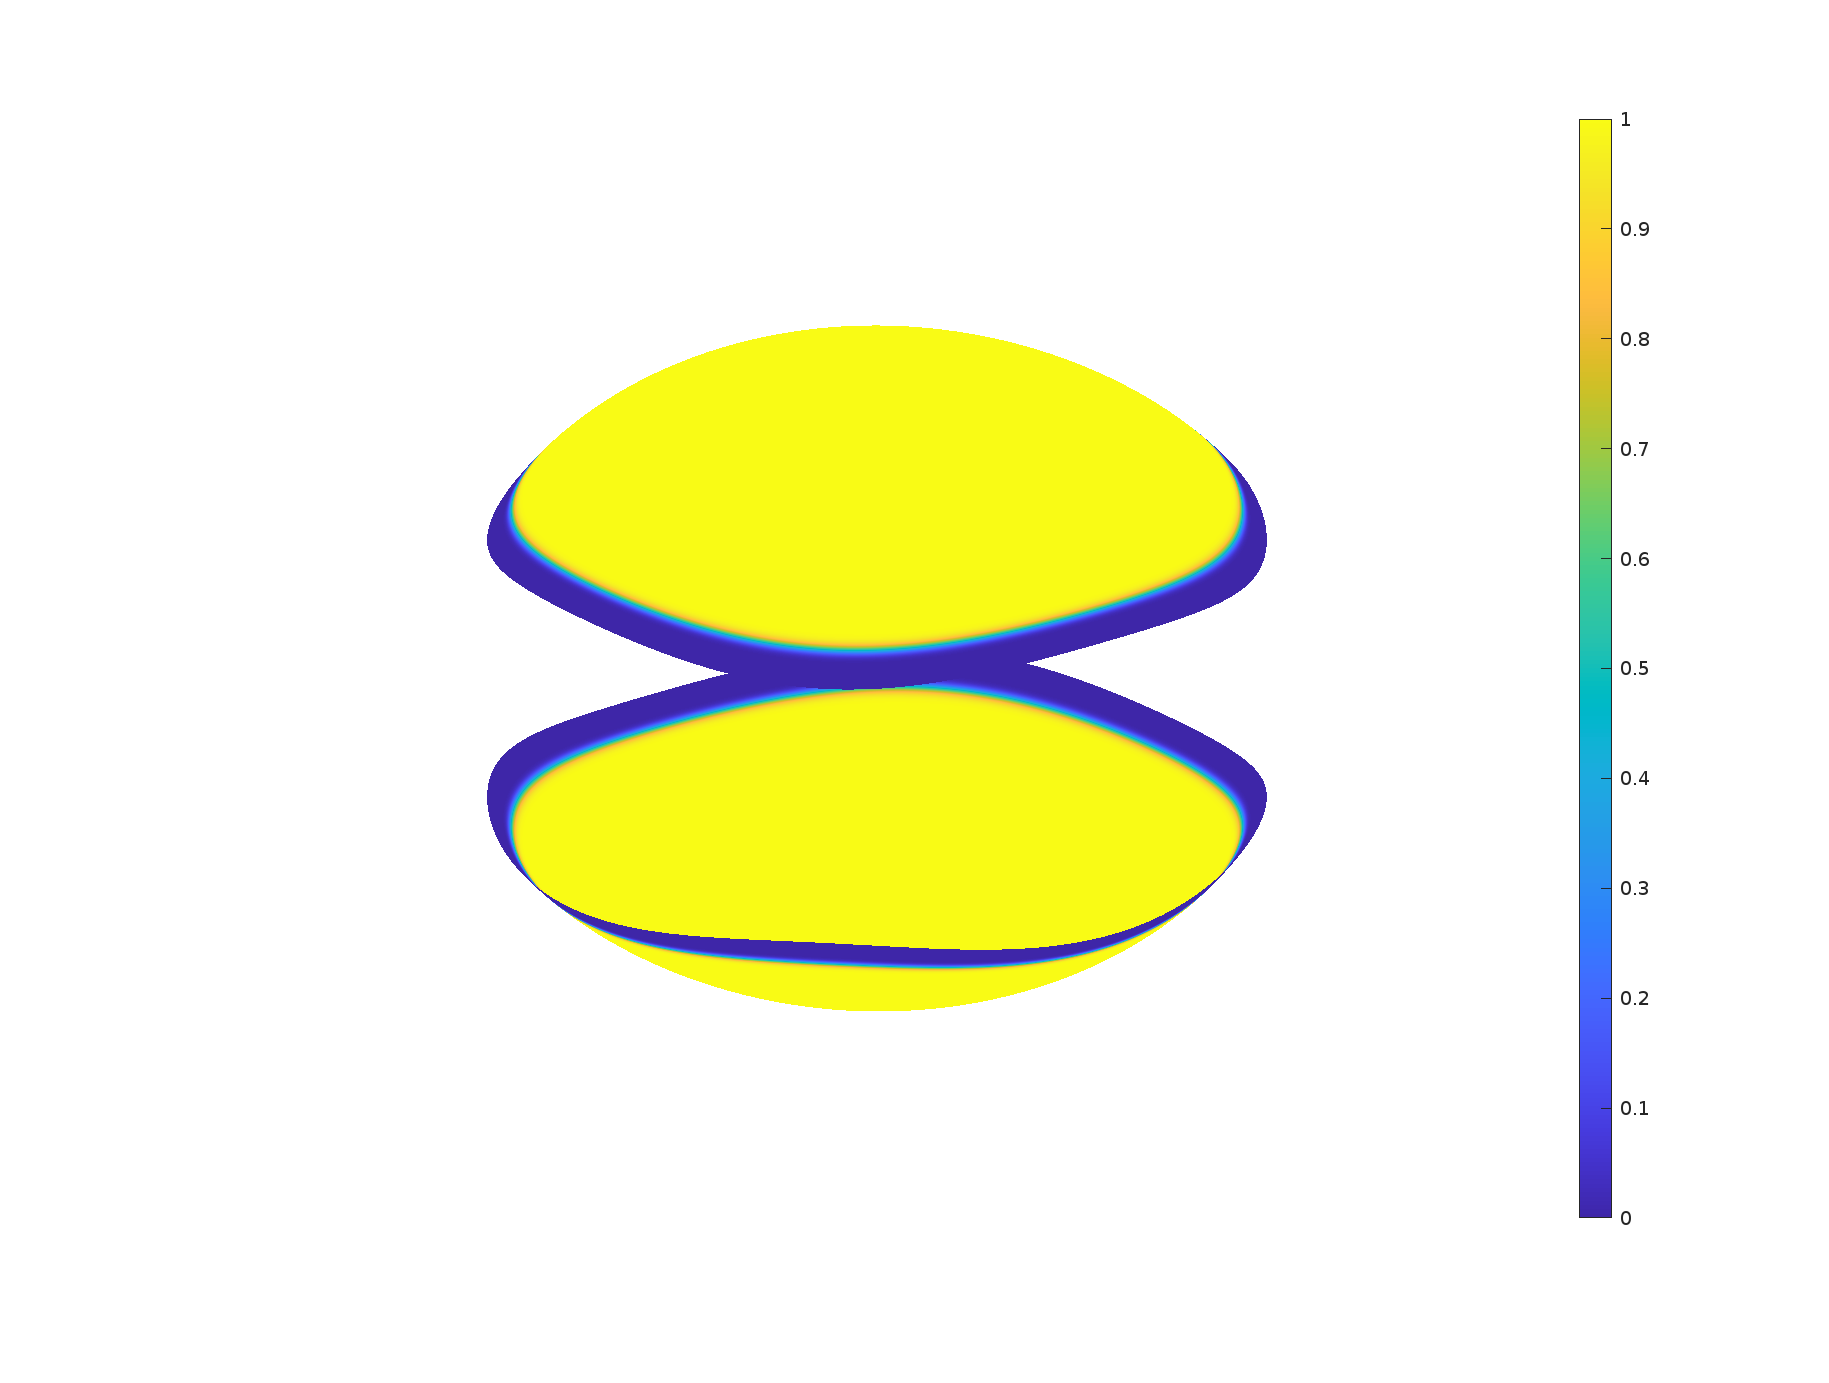
\includegraphics[scale = 0.2]{Images/PoO_03.eps}
            \caption{Die Karten \({\alpha_5}\) und \({\alpha_6}\).}
        \end{subfigure}
        \begin{subfigure}{0.49\textwidth}
            
\includegraphics[scale = 0.2]{Images/PoO_04.eps}
            \caption{Die Summe der \({\theta_i}\) auf \({M}\).}
            \label{fig:part_one:ex0:ex0:ex0}
        \end{subfigure}
        \caption{Die sechs Karten von \({\mathcal{M}}\) f\"ur \({p=4}\). Die Farbe beschreibt die Magnit\"ude der zugeh\"origen \({\theta_i}\).}
        \label{fig:part_one:ex0:ex0}
    \end{figure}

    \subsection{Visualisierung}
        Um eine gut konditionierte Parametrisierung von \({\mathcal{M}}\) (Abbildung \ref{fig:part_one:ex0:ex0:ex0}) zu erhalten wurde eine Einheitssph\"are parametrisiert (Kugelkoordinaten) und f\"ur jeden Punkt \({(x,y,z)^T\in S^2}\) das Newton-Verfahren auf die Funktion
        \[f(r)=\cos(rx)+\cos(ry)-(rz)^2-1\]
        angewandt, also einige Iterationen 
        \[r_{n+1}=r_n+\frac{\cos(r_nx)+\cos(r_ny)-(r_nz)^2-1}{x\sin(r_nx)+y\sin(r_ny)+2z^2r_n}\]
        mit \({r_0=\frac{\pi}{4}}\) berechnet. Da dieses gegen eine Nullstelle von \({f}\) konvergiert, konvergiert \({r_n\cdot(x,y,z)^T}\) gegen einen Punkt in \({\{\cos(x)+\cos(y)-z^2=1\}}\), also auch wahrscheinlich gegen einen Punkt in \({M}\). Auch wenn das Ergebnis aus der Perspektive wie eine Kugel aussieht, ist dies nicht der Fall. Die Visualisierung erfolgte in Matlab R2023a.